\documentclass{article}
\usepackage[utf8]{inputenc}
\usepackage{graphicx}
\usepackage{hyperref}
\usepackage{listings}
\usepackage{float}
\usepackage[french]{babel}
\begin{document}
\title{Données Séquentielles et Symboliques: Translittération automatique}

\author{Alexandre Bérard, Mathias Millet, Charles Robin}
\maketitle
\begin{abstract}
\end{abstract}
\vspace{0.5em}
\section{Introduction}

La translittération est le fait de traduire, entre deux langues dont les graphèmes diffèrent\footnote{Un graphème est l'unité de l'écrit correspondant au phonème, une unité de prononciation orale}, un mot ayant la même (ou presque) prononciation dans les deux langues. C'est surtout le cas pour le vocabulaire technique, qui conserve  la même prononciation entre plusieurs langues, mais dont la transcription va varier (en particulier lorsque les langues sont écrites avec des alphabets différents).

La translitération trouve un interêt lorsqu'elle est effectuée de manière automatique. En effet, avec l'aparition de nouveaux termes techniques, il est difficile de maintenir à jour des dictionnaires.\\


\subsection{Jeux de données}
Les données nous ont été fournies par Vincent Claveau. Nous disposons de deux jeux de données, concernant respectivement la translittération de l'\emph{espagnol} au \emph{portugais} et de l'\emph{anglais} vers le \emph{russe}. Chacun de ces jeux de données est divisé en deux fichiers, un fichier pour l'apprentissage et un fichier pour l'évaluation. Le fichier d'apprentissage contient plusieurs milliers d'entrées (3057 pour le portugais, et 7262 pour le russe), chaque entrée correspondant à un mot dans la langue originale et sa transcription dans le langage cible. Les entrées dans le fichier d'évaluation, elles, peuvent cependant contenir plusieurs transcriptions pour un même mot. 

\begin{figure}[H]
\caption{Entrées dans le fichier d'apprentissage Espagnol-Portugais}
\begin{verbatim}
2996: #fotocopiado# #fotocópia#
2997: #hexanoles# #hexanóis#
2998: #catalasa# #catalase#
\end{verbatim}
\end{figure}

\begin{figure}[H]
\caption{Entrées dans le fichier d'évaluation Espagnol-Portugais}
\begin{verbatim}
182: #centrifugación# #centrifugação#	other	unknown
183: #centriolo# #centríolo# OR #centríolos#	other	unknown
184: #ceramida# #ceramida# OR #ceramidas#	other	unknown
\end{verbatim}
\end{figure}

\subsection{Processus d'évaluation}
\paragraph{Ensembles de test et d'apprentissage}
Comme nous disposons de données de test et d'apprentissage, la question de la méthode d'échantillonage à utiliser ne se pose pas.

\paragraph{Métriques d'évaluation}
Nous devons choisir une métrique afin de mesurer les performances de nos classifieurs, et fournir une moyen de comparaison (avec d'autres classifieurs, une baseline, ou un opérateur humain).
Nous mesurons la précision de notre système, c'est à dire la proportion de mots correctement traduits.

\section{Règles de substitution}
Nous avons observé que dans le cas de l'espagnol et le portugais, les mots sont très similaires dans les deux langages. Dans les données d'apprentissage, la distance d'édition moyenne entre un mot espagnol et sa transcription en portugais est de \emph{2.0}.
Lorsque nous utilisons comme \emph{baseline} pour notre système de translittération, un système qui se contente de renvoyer le mot original, nous obtenons une précision de \emph{51.0\%} et une distance d'édition moyenne de \emph{1.06}.

\paragraph{}
Nous avons ensuite constaté qu'un système mettant en jeu les trois règles de substitution suivantes, obtenait une précision de \emph{58.6\%}, et une distance d'édition moyenne de \emph{0.76}.
\begin{verbatim}
is#->e#
ción#->ção#
ido#->ídeo#
\end{verbatim}

\section{Translittération statistique}
Le problème de la translittération est relativement proche de la traduction automatique. En traduction automatique, on traduit des séquences de mots d'un langage à un autre. Cela se caractérise par l'association à chaque mot (ou groupe de mots) de la phrase original, d'un mot (ou groupe de mots) dans le langage cible, avec un réordonnancement possible.

\begin{figure}[H]
\caption{Alignement de mots en traduction, et alignment de lettres en translittération}
\centering
\vspace{0.3cm}
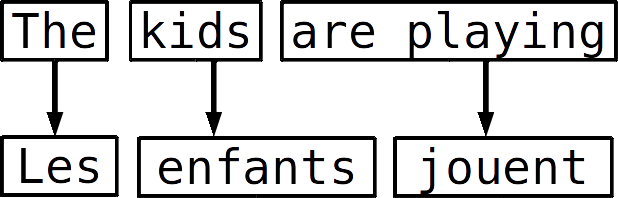
\includegraphics[scale=0.25]{word_alignment.png}
\hspace{0.5cm}
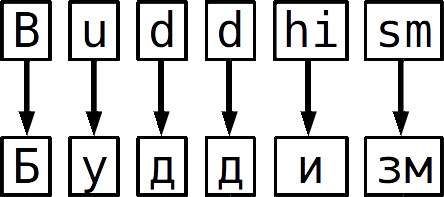
\includegraphics[scale=0.25]{letter_alignment.png}
\end{figure}

\section{Conclusion et perspectives}
\nocite{*}
\bibliographystyle{plain}
\bibliography{report}

\end{document}
